\chapter*{Animation}
\addcontentsline{toc}{chapter}{Animation}

For the animation, the subpackage \texttt{matplotlib.animation} has been used. The \texttt{FuncAnimation} function allows displaying consecutive plots as an animation. The robot is presented as a chain of two segments with dots at the extremities. The reference trajectory for the end-effector is plotted as a dashed line, allowing the motion to be appreciated from the beginning.

\begin{figure}[H]
    \centering
    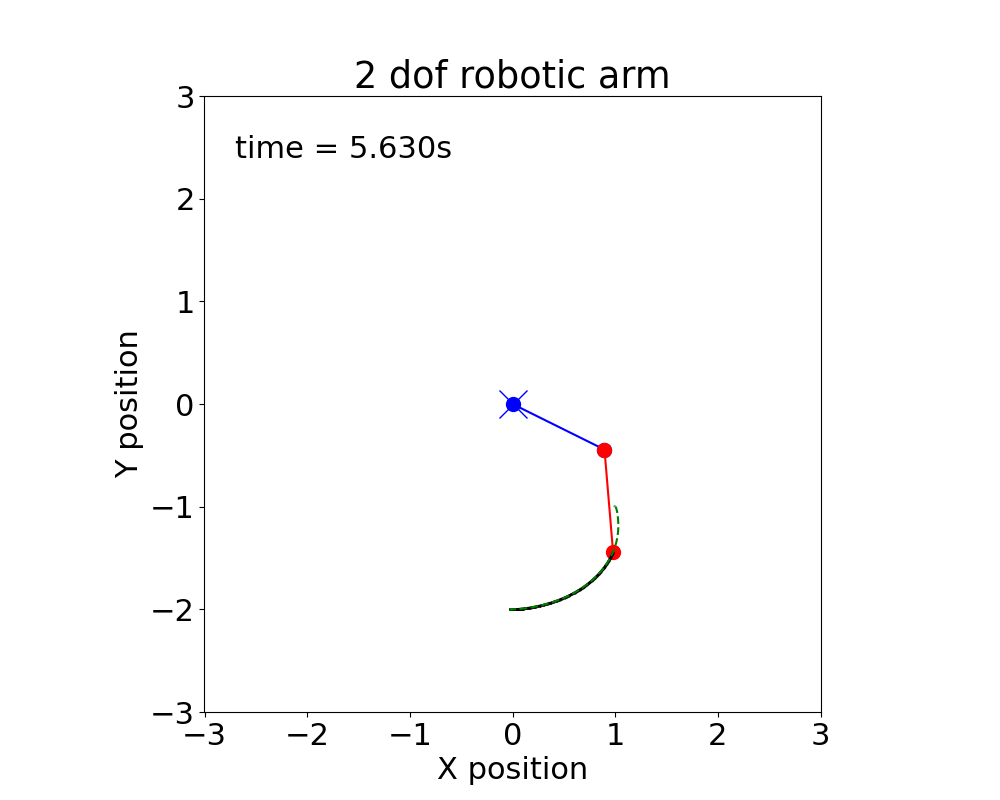
\includegraphics[width=0.8\linewidth]{figs/downward_video_0.png}
    \caption{Animation for the smooth trajectory of Task 2}
    \label{fig:downward_video_0}
\end{figure}


For the purpose of showing the various steps of the project, a simple trajectory has been presented in the previous figures. However, we have tested different trajectories that will be presented below with some plots and animations.

\subsection*{Swing up}

\begin{figure}[H]
    \centering
    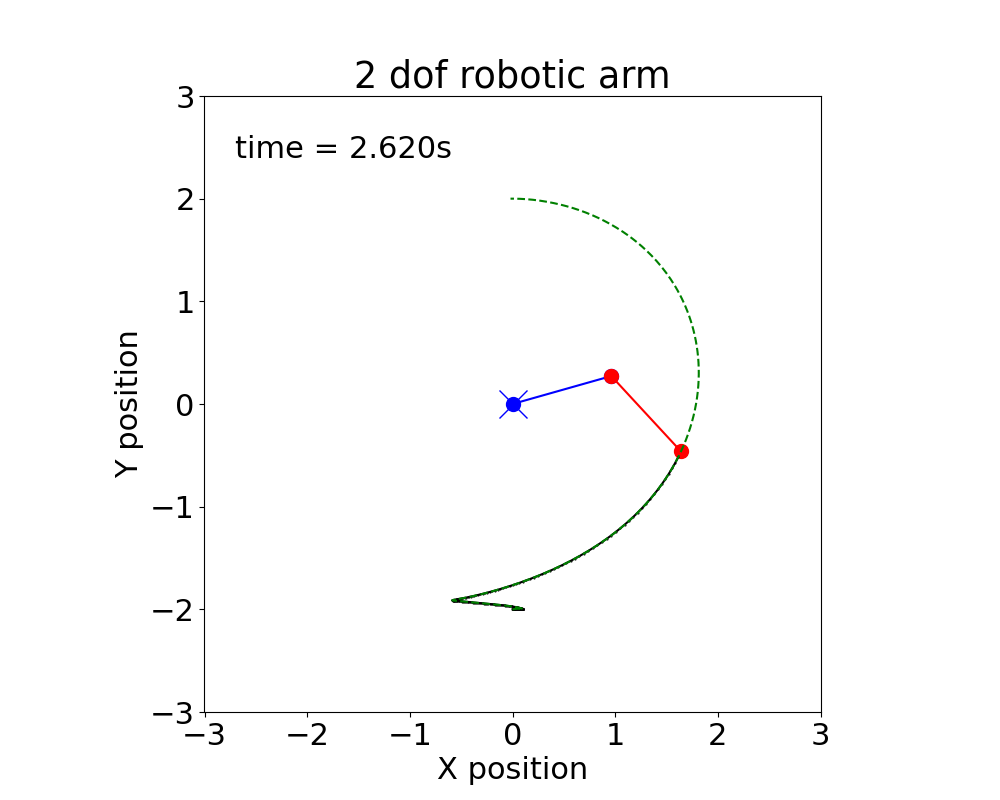
\includegraphics[width=0.8\linewidth]{figs/swing_video.png}
    \caption{Animation for the swing up trajectory}
    \label{fig:swing_video}
\end{figure}

\begin{figure}[H]
    \centering
    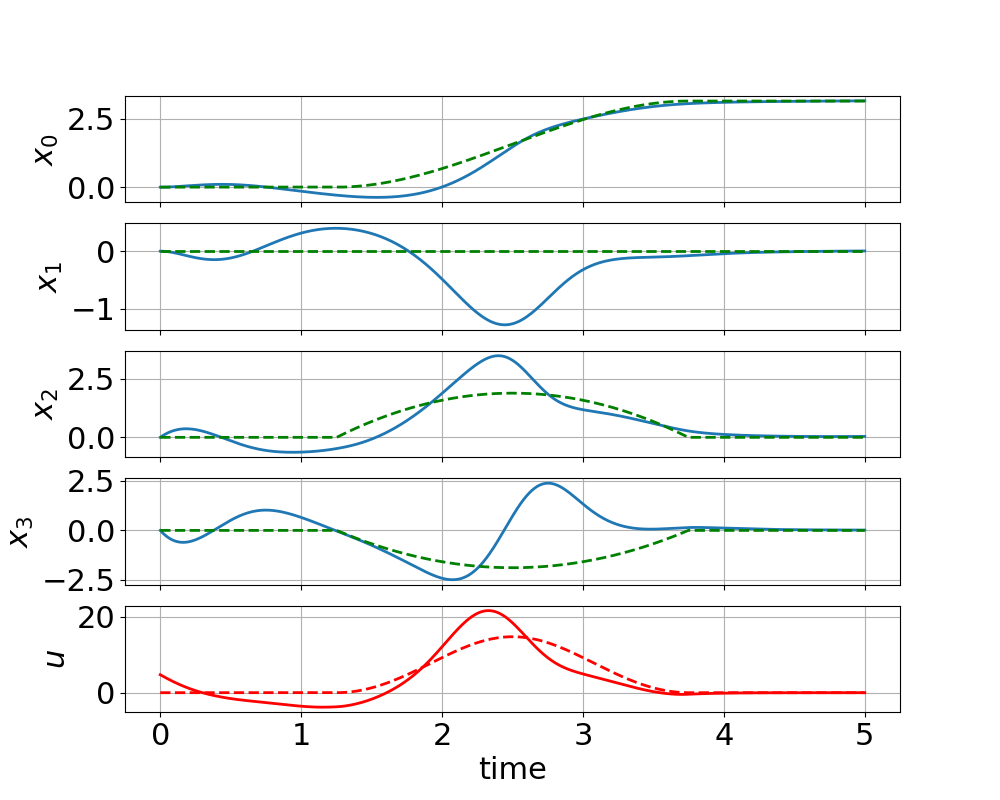
\includegraphics[width=0.8\linewidth]{figs/swing_result.png}
    \caption{Swing up final result}
    \label{fig:swing_result}
\end{figure}

\subsection*{Circular motion}

\begin{figure}[H]
    \centering
    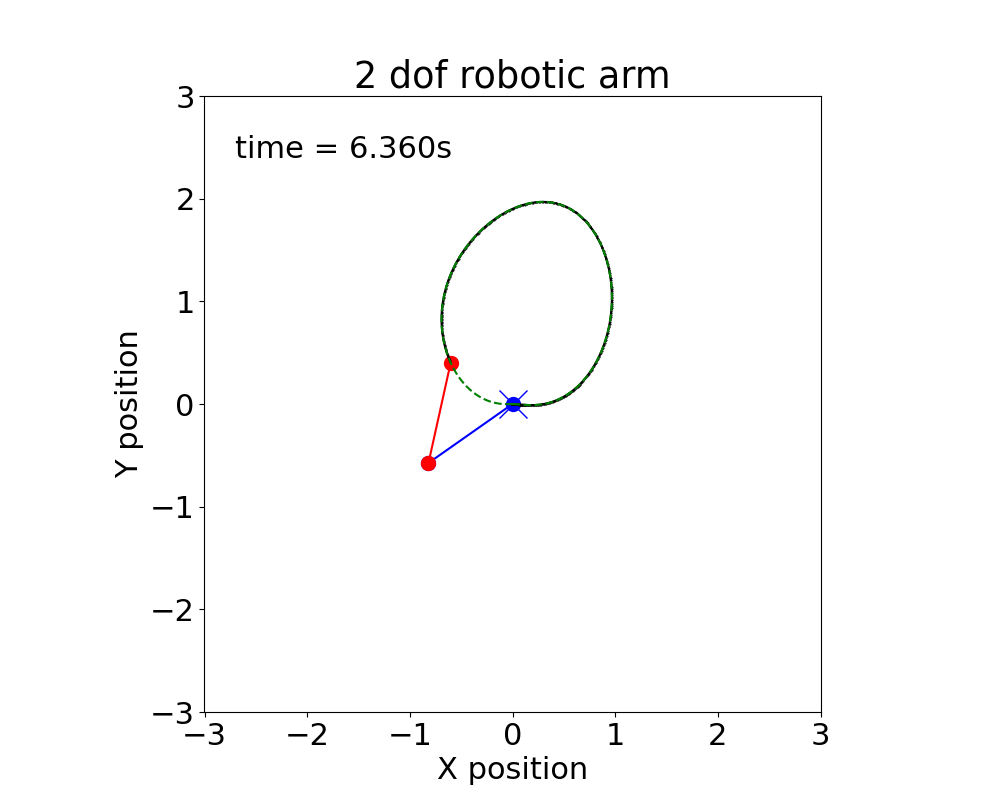
\includegraphics[width=0.8\linewidth]{figs/circle_video.png}
    \caption{Animation for the circular trajectory}
    \label{fig:swing_video}
\end{figure}

\begin{figure}[H]
    \centering
    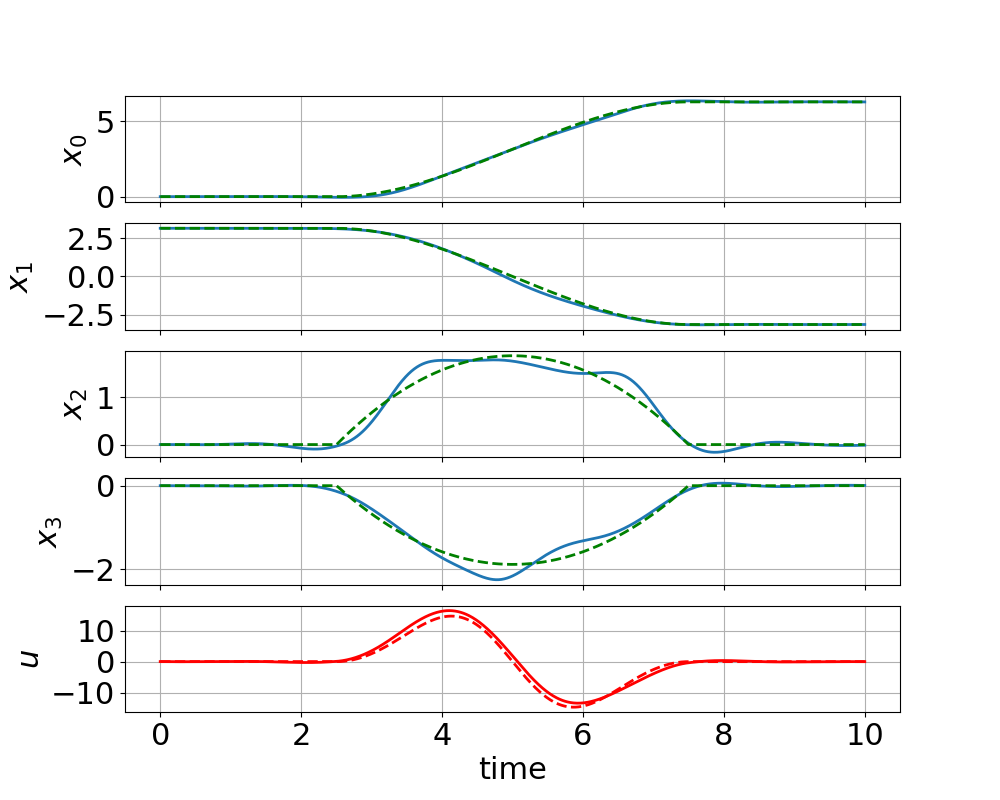
\includegraphics[width=0.8\linewidth]{figs/circle_result.png}
    \caption{Circular motion final result}
    \label{fig:circle_result}
\end{figure}